
Unless fully Lagrangian, one needs an additional numerical method to represent/track
the various materials present in an undeformable (Eulerian) mesh.

\todo[inline]{make a distinction between particle-in-cell and marker-and-cell}

\begin{center}
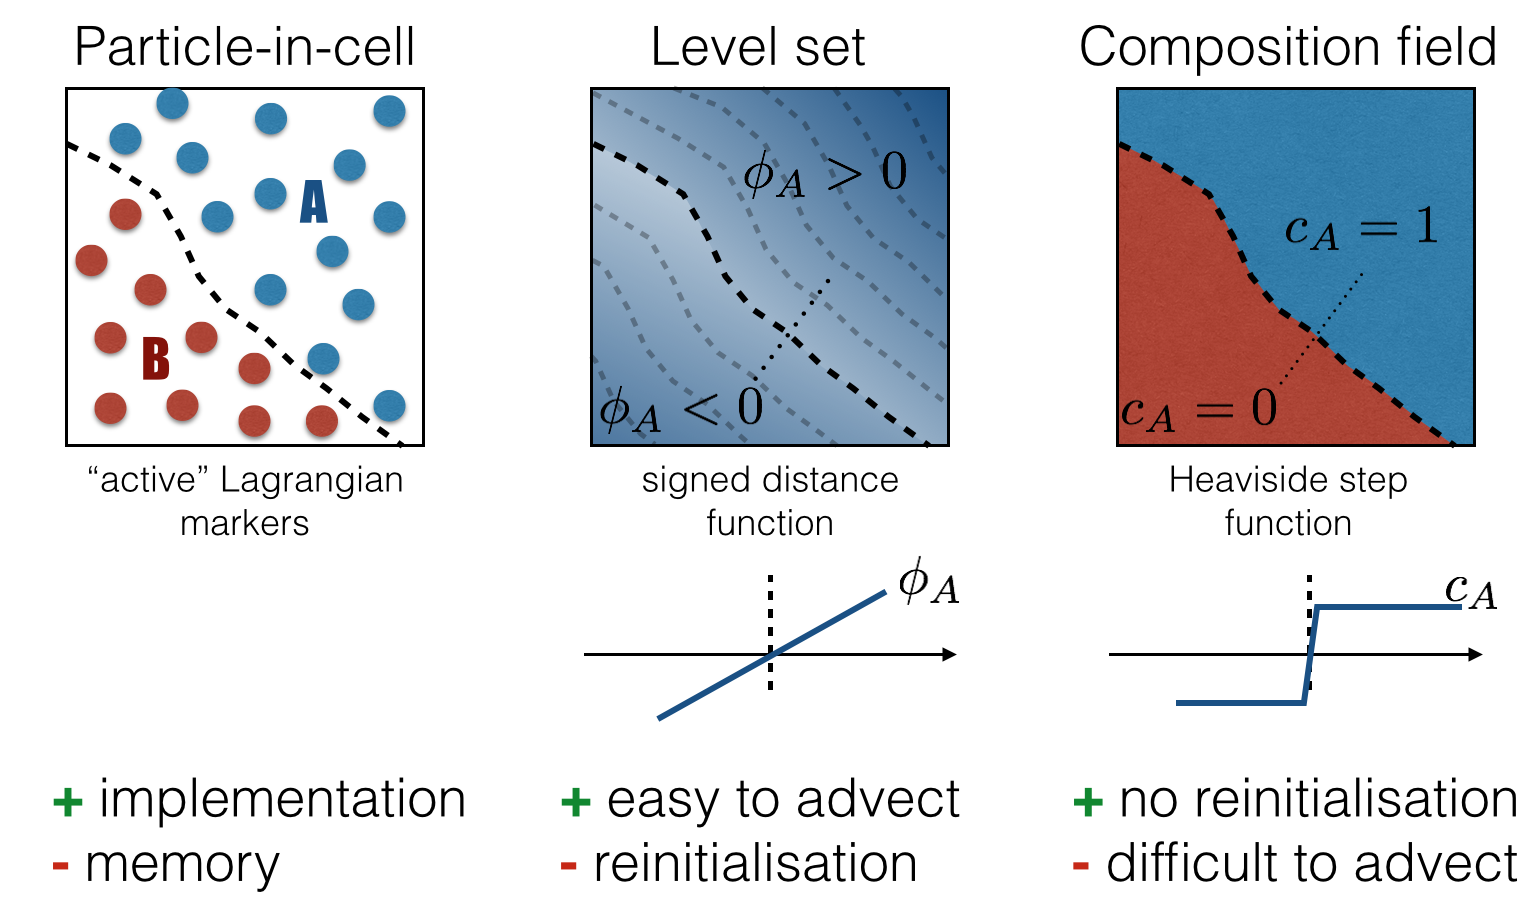
\includegraphics[width=15cm]{images/tracking}
\end{center}

%..............................................
\subsubsection{The Particle-in-cell technique}
\index{Particle in Cell}

\cite{galh19}

The Particle-in-cell method is widely used in the geodynamic literature \cite[e.g.][]{popo92}

 [Poliakov and Podladchikov, 1992; Moresi et al., 2003; Gerya and Yuen, 2003; McNamara and
Zhong, 2004; Popov and Sobolev, 2008; Thielmann et al., 2014]

It is the SOPALE, FANTOM, ELEFANT, I2/3(EL)VIS, ...

%..............................................
\subsubsection{The level set function technique}
\index{Level Set}


%..............................................
\subsubsection{The field/composition technique}
%\index{Field}

This is the approach taken by the ASPECT developers \cite{krhb12,hedg17}


%..............................................
\subsubsection{Hybrid methods}

Particle level sets \cite{brtf08}, \cite{saev10}



